\documentclass{guide}

\title{GPIO in Python}
\level{1}

\begin{document}
Het aansturen en uitlezen van de Raspberry-PI GPIO-pins kan op verschillende manieren. Wij gaan hiervoor python gebruiken en de library \texttt{RPi.GPIO}. Een library is een verzameling code die al door andere mensen is geschreven.

\section{Start van de code}
\label{sec:start_code}
Voordat we pinnen kunnen uitlezen of aansturen moeten we in python vertellen aan de Raspberry PI van welke library we gebruik maken, welke nummering van de pins we hanteren en welke pins we gaan gebruiken. In deze sectie bouwen we deze code op.

Codevoorbeeld \ref{code:importeer_library} laat zien hoe je de library \texttt{RPi.GPIO} importeert (regel 0) en hoe je vervolgens vertelt op welke nummering van de pinnen je gaat gebruiken (regel 2). Als je een functie wilt gebruiken van de library \texttt{RPi.GPIO} doe je dat door te starten met \enquote{\texttt{GPIO.}}. Op regel 2 is de functie \texttt{setmode} hier een voorbeeld van.

\begin{figure}[h]
  \centering
  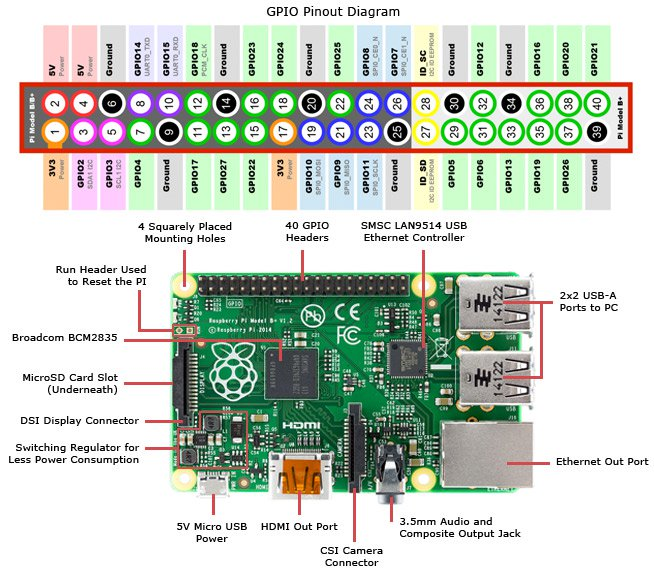
\includegraphics[width=\textwidth]{images/pinout.png}
  \caption{Pinout van de Raspberry Pi (bron: \href{https://www.jameco.com/Jameco/workshop/circuitnotes/raspberry-pi-circuit-note.html}{Jameco}).} \label{fig:pinout}
\end{figure}

De functie \texttt{setmode} vertelt welke nummering we gebruiken voor de pins. Er zijn twee opties: \texttt{GPIO.BCM} en \texttt{GPIO.BOARD}. Op Figuur~\ref{fig:pinout} zie we twee nummeringen. We zien de nummers in de grijze vierkanten en de nummers die beginnen met GPIO in de oranje rechthoeken. \texttt{GPIO.BOARD} geeft aan dat je de nummers in de grijze vierkanten gebruikt. \texttt{GPIO.BCM} geeft aan dat je de nummers in de oranje rechthoeken gebruikt.

\begin{python}[caption={De GPIO library inladen}, label=code:importeer_library]
import RPi.GPIO as GPIO

GPIO.setmode(GPIO.BCM)
\end{python}

\section{Code afsluiten}
\label{sec:afsluiten}
Als je de GPIO-pinnen gebruikt moet je je code netjes afsluiten. Je vertelt daarmee dat je programma niet meer gebruik maakt van de GPIO-pinnen en dat andere programma's er veilig gebruik van kunnen maken. Het afsluiten van je code doe je met de functie \enquote{GPIO.cleanup()} \footnote{Gebruik je dit niet \underline{of} beëindig je je programma voordat hij deze regel uitvoert, dan heb je de kans dat je een waarschuwing krijgt de volgende keer dat je je programma uitvoert. De Raspberry PI denkt dan dat je pinnen nog in gebruik zijn en waarschuwt hiervoor.}

\begin{python}[caption={De GPIO library inladen}, label=code:afsluiten]
GPIO.cleanup()
\end{python}

\section{Pin aansturen}
\label{sec:pin_aansturen}
Nu we weten hoe we de library toevoegen aan onze code en hoe we netjes de code moeten afsluiten kunnen we een GPIO-pin gaan aansturen. Hiervoor moeten we natuurlijk eerst een LED aansluiten.

\begin{figure}[ht]
\centering
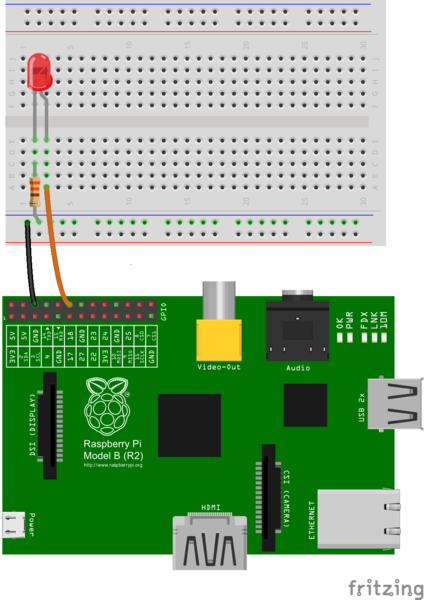
\includegraphics[scale=0.5]{images/PI_and_LED.png}
\caption{De aansluiting van een LED aan een Raspberry PI.} \label{fig:PI_and_LED}
\end{figure}

\subsection{Hardware}
Figuur~\ref{fig:PI_and_LED} laat zien hoe je een LED moet aansluiten op de Raspberry PI. Je hebt hiervoor nodig een breadboard, een LED, een weerstand(!) van minimaal $1k\Omega$ en DuPont kabels. Je kan een sterkere weerstand gebruiken, maar dit zal er voor zorgen dat de LED minder fel brandt.

\subsection{Code}
Codevoorbeeld \ref{code:PIN_aansturen} laat zien hoe je een GPIO-pin aanstuurt met python. Regel 0 en regel 3 hebben we besproken in sectie \ref{sec:start_code}. Regel 11 hebben we besproken in sectie \ref{sec:afsluiten}. Op regel 2 importeren we nog een extra library. De library \texttt{time} geeft ons de functie \texttt{sleep} die er voor zorgt dat onze code een bepaalde tijd wacht voordat het verder gaat. Het gebruik van deze functie zien we op regel 8.

Voordat we een GPIO-pin kunnen aansturen moeten we vertellen of we de pin gaan gebruiken als input-pin of als output-pin. Dit doen we op regel 5. Nu kunnen we pin 18 gebruiken als output-pin. Op regel 7 zetten we op de pin een hoog signaal. Op regel 9 zetten op de pin een laag signaal. 

\begin{python}[caption={De GPIO library inladen}, label=code:PIN_aansturen]
import RPi.GPIO as GPIO   # importeer library RPI.GPIO
import time               # importeer library time

GPIO.setmode(GPIO.BCM)    # zet de nummering op GPIO.BCM

GPIO.setup(18,GPIO.OUT)   # maak van pin 18 een output-pin

GPIO.output(18,GPIO.HIGH) # stuur een hoog signaal over pin 18.
time.sleep(1)             # wacht voor 1 seconde
GPIO.output(18,GPIO.LOW)  # stuur een laag signaal over pin 18.

GPIO.cleanup()            # sluit de code netjes af
\end{python}

\noindent De code van Codevoorbeeld \ref{code:PIN_aansturen} zet dus één keer de LED aan en daarna uit. Als je wilt dat hij dit vaker doet, dan kan je gebruik maken van een while of for-loop. Codevoorbeeld \ref{code:PIN_aansturen_for} laat de LED 10 keer knipperen. 

\begin{python}[caption={De GPIO library inladen}, label=code:PIN_aansturen_for]
import RPi.GPIO as GPIO     # importeer library RPI.GPIO
import time                 # importeer library time

GPIO.setmode(GPIO.BCM)      # zet de nummering op GPIO.BCM

GPIO.setup(18,GPIO.OUT)     # maak van pin 18 een output-pin

for i in range(10):
  GPIO.output(18,GPIO.HIGH) # stuur een hoog signaal over pin 18.
  time.sleep(1)             # wacht voor 1 seconde
  GPIO.output(18,GPIO.LOW)  # stuur een laag signaal over pin 18.
    time.sleep(1)           # wacht voor 1 seconde

GPIO.cleanup()              # sluit de code netjes af
\end{python}

\noindent Een output-pin kan je gebruiken om een LED aan te sturen, maar je kan hem ook gebruiken om andere hardware aan te sturen (bijvoorbeeld een buzzer of een speaker) of om informatie te sturen naar een andere Raspberry PI.

\section{Pin uitlezen}
\label{sec:pin_uitlezen}
We gaan in deze sectie kijken hoe we een GPIO-pin uitlezen. Dit doen we door een knopje aan te sluiten.

\subsection{Hardware}
Figuur~\ref{fig:PI_and_button} laat zien hoe je een knopje aansluit. Hiervoor heb je nodig een breadboard, een knopje en DuPont-kabels. We hebben geen weerstand nodig, want voor input kan de Raspberry PI een interne weerstand gebruiken. Dit moeten we wel aangeven in de code!

\begin{figure}[ht]
\centering
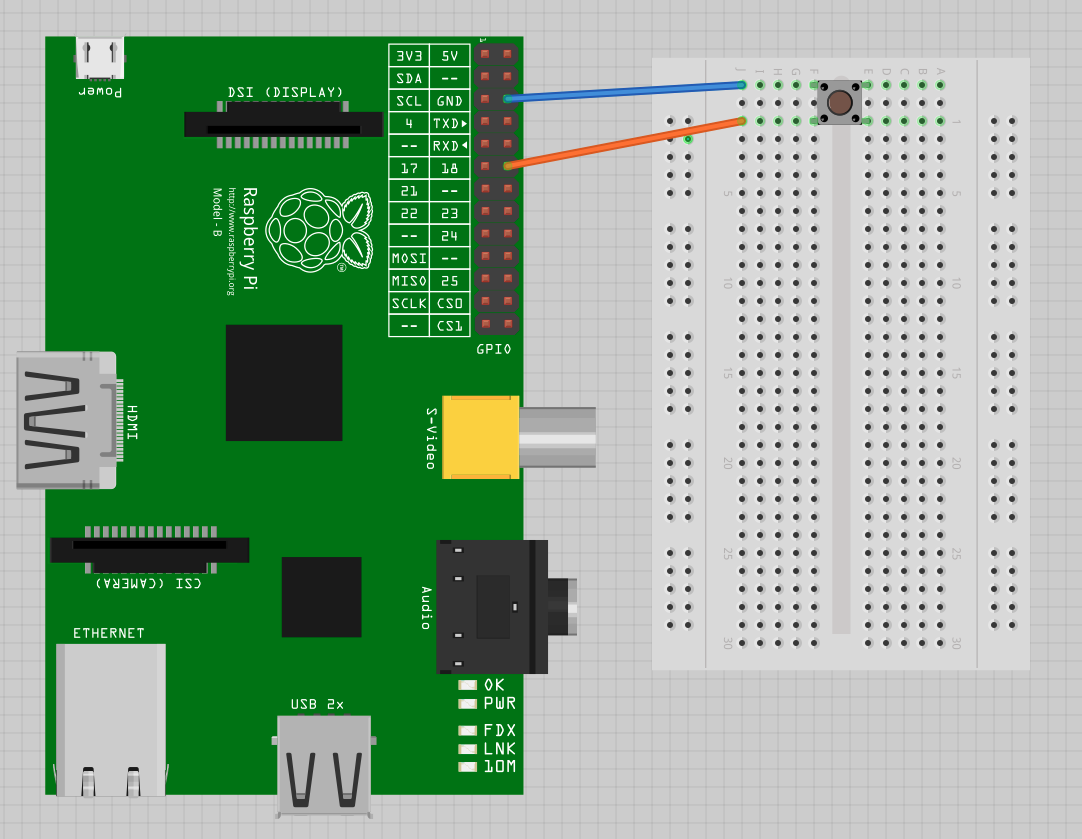
\includegraphics[scale=0.6]{images/PI_and_button.png}
\caption{De aansluiting van een button aan een Raspberry PI.} \label{fig:PI_and_button}
\end{figure}

\subsection{Code}
Codevoorbeeld \ref{code:PIN_uitlezen} laat zien hoe je een knop kan uitlezen. Op regel 5 zeggen we dat pin 18 een input-pin is en dat hij de interne weerstand moet gebruiken (\enquote{\texttt{pull\_up\_down=GPIO.PUD\_UP}}). Vervolgens kunnen we met de functie \enquote{\texttt{GPIO.input(18)}} de input van pin 18 uitlezen. Dit doen we op regel 10. Op deze regel stoppen we deze input in de variabele \enquote{input\_state}\footnote{De variabele \enquote{\texttt{input\_state}} is niet per s\'{e} nodig. De code zou ook werken als we de functie \enquote{\texttt{GPIO.input(18)}} direct gebruiken in de if-statement op regel 12.}. Deze variabele is van het type \texttt{bool}.

De variabele \enquote{\texttt{input\_state}} kunnen we nu gebruiken in een if-statement. Dit doen we op regel 12. Tegen intu\"{i}tie in geeft de functie \enquote{\texttt{GPIO.input(18)}} de waarde \texttt{False} wanneer de knop is ingedrukt! Door in de if-statement \enquote{\texttt{not}} te gebruiken controleren we of \enquote{\texttt{input\_state}} de waarde \texttt{False} heeft en daarmee of de knop is ingedrukt.

\begin{python}[caption={De GPIO library inladen}, label=code:PIN_uitlezen]
import RPi.GPIO as GPIO           # importeer library RPi.GPIO
import time                       # importeer library time

GPIO.setmode(GPIO.BCM)            # zet de nummering op GPIO.BCM

# Maak van pin 18 een input-pin en maak gebruik van de interne weerstand
GPIO.setup(18, GPIO.IN, pull_up_down=GPIO.PUD_UP) 

for i in range(500):              # Herhaal het onderstaande 1000 keer
    input_state = GPIO.input(18)  # lees pin 18 uit en sla het op in de
                                  # variabele input_state
    if not input_state:           # als de knop is ingedrukt
        print('Button Pressed')   # print op het scherm
        time.sleep(0.1)           # wacht voor 0.1 seconden
  else:                           # als niet op is gedrukt
      print('Button not Pressed') # print op het scherm
        time.sleep(0.1)           # wacht voor 0.1 seconde

GPIO.cleanup()                    # sluit de code netjes af
\end{python}

\end{document}
